\chapter{Experimental Setup}\label{ch:experimentalsetup}
All our experiments are quantitative experiments, measured over a corpus using CloneRefactor. In this chapter, we first explain the corpus we use. We then explain how we calculate the impact of refactorings on the software maintainability.

\section{The Corpus}\label{chap:corpus}
For our experiments we use a large corpus of open-source projects assembled by Allamanis et al.~\cite{githubCorpus2013}\footnote{The corpus can be downloaded at: \url{http://groups.inf.ed.ac.uk/cup/javaGithub/}}. This corpus contains a set of Java projects from GitHub, selected by the number of forks. The projects and files in this corpus were de-duplicated manually. This results in a variety of Java projects that reflect the quality of average open-source Java systems and are useful to perform measurements on.

Because CloneRefactor requires all dependencies for the projects it analyses, we created a set of scripts\footnote{All scripts to prepare the corpus are available on GitHub: \url{https://github.com/SimonBaars/GitHub-Java-Corpus-Scripts}} to filter the corpus for all projects for which we can obtain all dependencies using Maven. In this section, we explain the actions performed by the scripts and the rationale behind those actions.

\subsection{Filtering Maven projects}
As explained in Section~\ref{chap:challenge}, CloneRefactor requires all the libraries a software project is dependent on to perform its clone analysis. As these are not included in the corpus by Allamanis \cite{githubCorpus2013}, we created a script to gather these dependencies. As Java projects manage their dependencies in many different ways, we decided to limit our scope to a single build automation system. We chose Maven, as it is one of the most used build automation systems for Java projects. Maven uses a file, named \texttt{pom.xml}, to describe a projects' dependencies. Our script clones the latest version of each project in the corpus. It then removes each project that has no \texttt{pom.xml} file (which indicates that those projects do not use the Maven build automation system).

We then continued to filter all test code and generated files. As many projects store these files in many different places, we decided to further filter the corpus to only include projects with a conventional structure. When using Maven, projects are recommended to put their production code in the folder structure \texttt{src/main/java}. We omitted Maven projects that do not adhere to this convention. We instruct CloneRefactor only to use the sources in the \texttt{src/main/java} folder. This decreases the chance of generated files and test code being considered for clone detection.

\subsection{Gathering Dependencies}
As a next step, we collect all dependencies of the downloaded software projects. Maven uses the following command to automate this process: \texttt{mvn dependency:copy-dependencies -DoutputDirectory=lib}. This process fails if the project requires external dependencies that are no longer available. Our scripts remove such projects for which it cannot obtain all dependencies.

\subsection{Building an AST of all Java files}
To verify the syntactical correctness of all Java files in the projects, we used JavaParser \cite{tomassetti2017javaparser} to create an AST of every Java file in the \texttt{src/main/java} folder of the software projects. A very small set of projects had syntactical errors, which we removed from the corpus. For instance, some projects had code that was still in development on their \textit{master} branch, which did not compile. We remove them because CloneRefactor cannot parse them into an AST.

\subsection{Inspecting outliers}
We ran CloneRefactor over every project in the corpus and inspected the output for each project. Some projects gave unusual high numbers of clones of a certain size, which we manually inspected. Often these projects contained generated source files. We removed these projects from the corpus.

\subsection{Resulting corpus}
This procedure results in 2,267 Java projects including all their dependencies\footnote{The full list of projects is in the following file in our GitHub repository: \url{https://github.com/SimonBaars/GitHub-Java-Corpus-Scripts/blob/master/filtered_projects.txt}}. The projects vary in size and quality. The total size of all projects is 14.210.357 lines (11,315,484 when excluding whitespace) over a total of 99,586 Java files. This is an average of 6,268 lines over an average of 44 files per project, 141 lines on average per file. The largest project in the corpus is \textit{VisAD} with 502,052 lines over 1,527 files. The distribution of project sizes is displayed in Fig.~\ref{fig:dist}.

\begin{figure}[H]
  \centering
  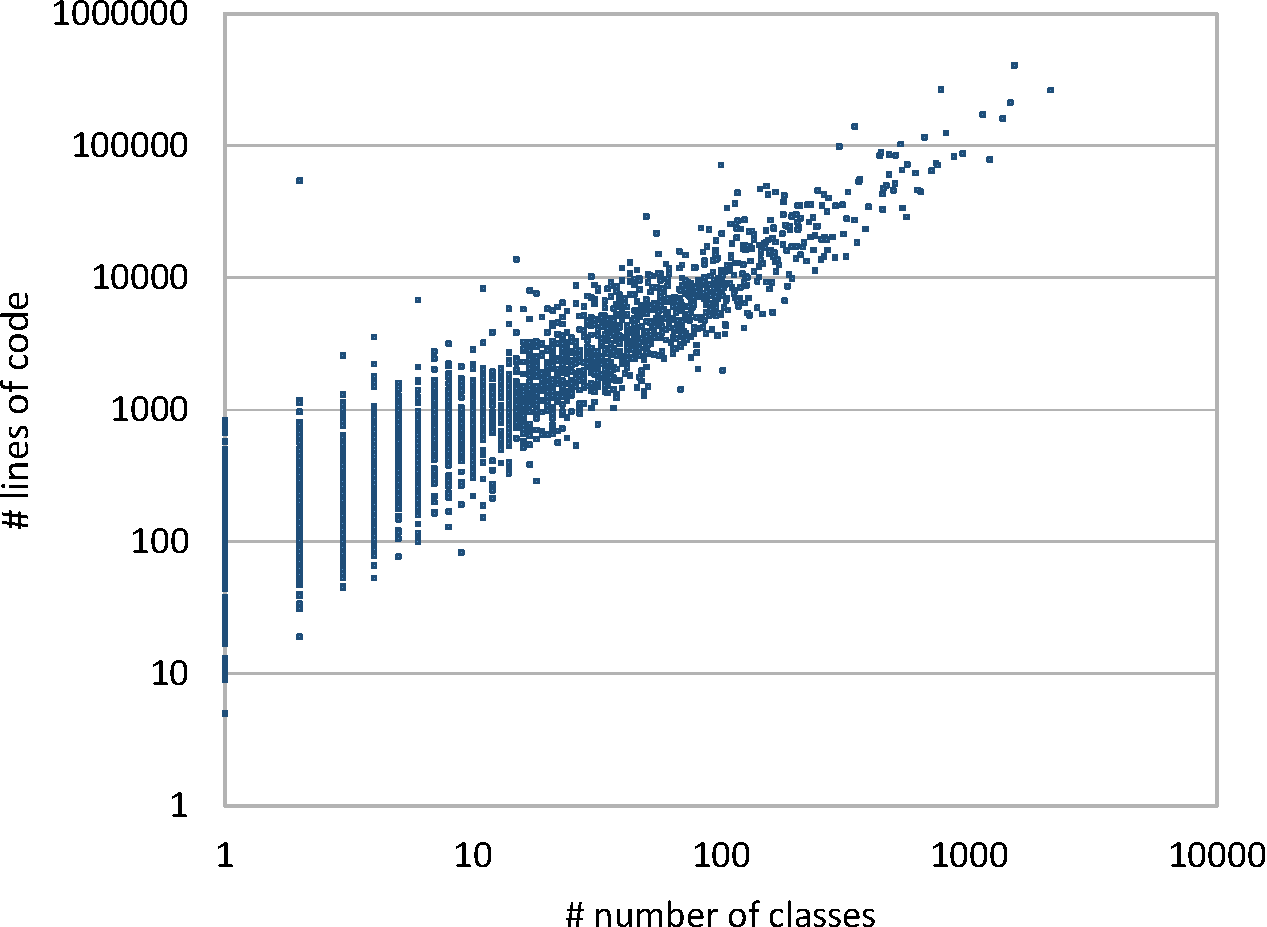
\includegraphics[width=0.65\columnwidth]{img/dist2}
  \caption{Distribution of project sizes in corpus on a logarithmic scale.}
  \label{fig:dist}
\end{figure}

\section{Tool Validation}
We have validated the correctness of CloneRefactor through unit tests and empirical validation. First, we created a set of 57 control projects\footnote{Control projects for testing CloneRefactor: \url{https://github.com/SimonBaars/CloneRefactor/tree/master/src/test/resources}} to verify the correctness in many (edge) cases. These projects test each identified relation, location, contents and refactorability category (see Section \ref{chap:contextsetup} and \ref{sec:refactorabilitysetup}), to see whether they are correctly identified. Next, we run the tool over the corpus and manually verify samples of the acquired results. This way, we check the correctness of the identified clones, their context, and their proposed refactoring.

We also test the correctness of the resulting code after refactoring. For this, we use a project named JFreeChart\footnote{JFreeChart is available on GitHub: \url{https://github.com/jfree/jfreechart}}. JFreeChart has high test coverage and working tests, which allows us to test the correctness of the program after running CloneRefactor. We run CloneRefactor manually over the JFreeChart project, run its test cases and check the correctness of the proposed refactorings.

\section{Minimum clone size}
In this study, we want to find out what thresholds will improve maintainability if clones by those thresholds are refactored. For example, when clones are very small, refactoring them might not improve maintainability since the detrimental effect of the added volume of the newly created method exceeds the positive effect of removing duplication. Because of that, we perform all our experiments with a minimum clone size of 10 tokens, because smaller clones almost never improve maintainability when refactored.

The reason for this is that when applying the ``Extract Method'' refactoring technique, we create a new method. An empty method in Java consists of 7 tokens. We also need calls to the extracted method, which is 4 tokens per call if no parameters/arguments are required. Empirically, we found all clones below 10 tokens in size, are very unlikely to affect maintainability positively. To avoid such clones polluting our data, we do not consider clones smaller than 10 tokens.

\section{Calculating a maintainability score}\label{sec:metricformula}
In this study, we use four metrics to determine maintainability (see Section~\ref{sec:metrics}). For each of these metrics, we collect their increase/decrease (delta) after each applied refactoring. We aggregate these delta metric values to draw a conclusion about the maintainability increase or decrease after applying a refactoring. We base our aggregation on the following assumptions:
\begin{itemize}
  \item All metrics are equal in terms of weight towards system maintenance effort.
  \item Higher values for the metrics imply lower maintainability.
  \item Normalizing each obtained metric delta over all deltas obtained for that metric in our dataset results in equally weighted scores.
\end{itemize}
We derived these assumptions from supporting evidence shown by Heitlager et al~\cite{heitlager2007practical} and Alves et al.~\cite{alves2010deriving}. Using the resulting aggregated maintainability score, we can argue for each refactoring whether it increases or decreases the maintainability of the system.

We normalize each obtained metric delta using the ``Standard score'', which is calculated as follows:
\begin{equation}\label{eq:scoredev}
N_{metric} = \frac {\Delta X-\mu}{\sigma}
\end{equation}
Where $\Delta X$ is a metric delta, $\mu$ is the mean of all deltas for this metric and $\sigma$ is the standard deviation of all deltas for this metric. This method works well for normalization of our data because it is resilient against outliers. We divide by the standard deviation so outliers do not influence the resulting scores much.

We then calculate the maintainability score for a specific refactoring as follows:
\begin{equation}\label{eq:scoreref}
\text{Maintainability Score} = N_{duplication} + N_{complexity} + N_{volume} + N_{parameters}
\end{equation}
